\documentclass[11pt,a4paper]{article}

\usepackage{amsmath,amssymb}
\usepackage{graphicx}
\usepackage{booktabs}
\usepackage[margin=2.5cm]{geometry}
\usepackage{caption}
\usepackage[colorlinks=true,linkcolor=blue,citecolor=blue,urlcolor=blue]{hyperref}

\graphicspath{{../figures/}}

% ---------- Macros ----------
\newcommand{\ket}[1]{\left|#1\right\rangle}
\newcommand{\bra}[1]{\left\langle #1\right|}
\newcommand{\braket}[2]{\left\langle #1\middle|#2\right\rangle}
\newcommand{\Tr}{\operatorname{Tr}}
\newcommand{\Var}{\operatorname{Var}}
\newcommand{\FQ}{F_Q}

% Two figures side by side: \figpair{left file}{right file}{caption}
\newcommand{\figpair}[3]{%
  \begin{figure}[htbp]
    \centering
    \includegraphics[width=0.48\textwidth]{#1}\hfill
    \includegraphics[width=0.48\textwidth]{#2}
    \caption{#3}
  \end{figure}}

% One centred figure: \figone{file}{caption}
\newcommand{\figone}[2]{%
  \begin{figure}[htbp]
    \centering
    \includegraphics[width=0.62\textwidth]{#1}
    \caption{#2}
  \end{figure}}

\title{Entanglement Dynamics and Quantum Metrology\\in a Two-Qubit Heisenberg XXZ Model}
\author{Dhimen Nabil\\[2pt]
\small Master in Mathematical Physics, Faculty of Sciences, Mohammed V University, Rabat\\
\small LPHE -- Mod\'elisation et Simulation}
\date{}

\begin{document}
\maketitle

\begin{abstract}
We study the time evolution of entanglement, reduced-state purity and quantum Fisher information (QFI) in a two-qubit Heisenberg XXZ model. Four initial pure states are chosen so that they cover the symmetry sectors of the Hamiltonian: a stationary product state, a product state that becomes maximally entangled, a product state that generates partial entanglement, and a stationary maximally entangled state. Entanglement is quantified by concurrence and negativity, and the mixedness of each qubit by the purity of its reduced state. For the metrological part, the Hamiltonian is perturbed by $\lambda V$ with $V$ the total $S_z$, and the QFI and the Cram\'er--Rao bound on the estimation of $\lambda$ are obtained analytically and checked numerically. Because the total $S_z$ is conserved, the anisotropy $\Delta$ only enters as a phase and the QFI reduces to $4t^2\Var(V)$; we discuss what this means for entanglement as a metrological resource. In a last part, the generator is replaced by the total $S_x$, which does not commute with the Hamiltonian, and each qubit is subject to local dephasing described by a Lindblad equation. Then $\Delta$ enters the QFI through the detuning $2J(1-\Delta)$, the Bell state gives twice the QFI of the product states $\ket{00}$ and $\ket{01}$ without noise, and this advantage shrinks but survives at the best interrogation time as the dephasing rate grows; no sudden death of entanglement occurs, and at long times $\ket{00}$, $\ket{01}$ and $\ket{\psi_+}$ reach the same QFI plateau, so the advantage disappears.
\end{abstract}

\tableofcontents
\newpage

% ====================================================================
\section{Introduction}
% ====================================================================

Heisenberg-type spin models are the simplest interacting quantum systems in which entanglement is generated dynamically, and they are a standard testbed for quantum information protocols. In the two-qubit case the dynamics can be solved in closed form, which makes it possible to compare analytic results with numerical simulations and to understand exactly which feature of the model controls each quantity.

The report is organised as follows. Section~\ref{sec:prelim} recalls the entanglement measures and the metrological tools used throughout. Section~\ref{sec:dynamics} formulates the XXZ model, diagonalises it, and studies concurrence, negativity and purity for four initial states. Section~\ref{sec:metrology} introduces the metrological parameter and computes the QFI and the Cram\'er--Rao bound for the same states. Section~\ref{sec:noncomm} replaces the generator by one that does not commute with $H$ and adds local dephasing. Section~\ref{sec:conclusion} concludes and gives perspectives. The hand calculations and the numerical implementation are in the appendices.

% ====================================================================
\section{Preliminaries}\label{sec:prelim}
% ====================================================================

\subsection{Entanglement measures}

For a pure two-qubit state $\ket{\psi}=c_{00}\ket{00}+c_{01}\ket{01}+c_{10}\ket{10}+c_{11}\ket{11}$ the concurrence is
\begin{equation}
  C(\psi)=2\,\lvert c_{00}c_{11}-c_{01}c_{10}\rvert .
\end{equation}
For a general mixed state $\rho$, Wootters' formula is $C(\rho)=\max\{0,\mu_1-\mu_2-\mu_3-\mu_4\}$, where $\mu_i$ are the square roots, in decreasing order, of the eigenvalues of $\rho\tilde\rho$, with $\tilde\rho=(\sigma_y\otimes\sigma_y)\rho^{*}(\sigma_y\otimes\sigma_y)$ \cite{Wootters1998}.

The negativity used here is the sum of the absolute values of the negative eigenvalues of the partial transpose,
\begin{equation}
  \mathcal N(\rho)=\sum_{\mu_i<0}\lvert\mu_i\rvert,\qquad \mu_i\in\operatorname{spec}\bigl(\rho^{T_B}\bigr),
\end{equation}
which equals $(\lVert\rho^{T_B}\rVert_1-1)/2$ \cite{VidalWerner2002}.

\paragraph{Relation between $\mathcal N$ and $C$ for pure states.}
Let the Schmidt coefficients of a pure two-qubit state be $\lambda_{1,2}$ with $\lambda_1+\lambda_2=1$. The eigenvalues of $\rho^{T_B}$ are $\lambda_1$, $\lambda_2$ and $\pm\sqrt{\lambda_1\lambda_2}$, so $\mathcal N=\sqrt{\lambda_1\lambda_2}$. Since $C=2\sqrt{\lambda_1\lambda_2}$, we obtain
\begin{equation}
  \mathcal N=\frac{C}{2}\quad\text{for every pure two-qubit state.}
\end{equation}

\subsection{Purity of the reduced states}

The purity of the reduced state of qubit $A$ is $P_A=\Tr\rho_A^2$, and similarly for $B$. For a global pure state, $\rho_A$ and $\rho_B$ share the same spectrum $\{\lambda_1,\lambda_2\}$, hence $P_A=P_B=\lambda_1^2+\lambda_2^2=1-2\lambda_1\lambda_2$, that is
\begin{equation}
  P_A=P_B=1-\frac{C^2}{2}.
  \label{eq:purity-C}
\end{equation}
Purity is $1$ for a product state and $1/2$ for a maximally entangled one.

\subsection{Quantum Fisher information and the Cram\'er--Rao bound}

Let a pure state $\ket{\psi_\lambda}$ depend on an unknown parameter $\lambda$. Its quantum Fisher information is
\begin{equation}
  \FQ=4\left(\braket{\partial_\lambda\psi_\lambda}{\partial_\lambda\psi_\lambda}-\bigl\lvert\braket{\psi_\lambda}{\partial_\lambda\psi_\lambda}\bigr\rvert^2\right),
\end{equation}
and for $N$ independent repetitions any unbiased estimator obeys the quantum Cram\'er--Rao bound \cite{BraunsteinCaves1994,Giovannetti2011}
\begin{equation}
  \delta\lambda\ \ge\ \delta\lambda_{\min}=\frac{1}{\sqrt{N\,\FQ}}.
\end{equation}
Saturating the bound requires an optimal measurement; the bound itself only depends on the state family.

% ====================================================================
\section{Entanglement and Purity Dynamics in the XXZ Model}\label{sec:dynamics}
% ====================================================================

\subsection{Introduction and formulation of the model}

\subsubsection{Hamiltonian}
We use $\hbar=1$ and
\begin{equation}
  H=J\left(\sigma_x\otimes\sigma_x+\sigma_y\otimes\sigma_y+\Delta\,\sigma_z\otimes\sigma_z\right),
\end{equation}
where $\sigma_{x,y,z}$ are Pauli matrices (not spin-$1/2$ operators), $J$ is the coupling and $\Delta$ the anisotropy. Numerically $J=1$, $\Delta=0.5$ and $t\in[0,2\pi]$. Using Pauli matrices rather than $S=\sigma/2$ means that the characteristic frequency is $4J$.

\subsubsection{Matrix form in the computational basis}
In the ordered basis $\{\ket{00},\ket{01},\ket{10},\ket{11}\}$, using $\sigma_x\otimes\sigma_x+\sigma_y\otimes\sigma_y=2\bigl(\ket{01}\!\bra{10}+\ket{10}\!\bra{01}\bigr)$,
\begin{equation}
  H=J\begin{pmatrix}
  \Delta&0&0&0\\
  0&-\Delta&2&0\\
  0&2&-\Delta&0\\
  0&0&0&\Delta
  \end{pmatrix}.
\end{equation}

\subsubsection{Eigenvalues and eigenvectors}
\begin{table}[htbp]
  \centering
  \begin{tabular}{@{}lcc@{}}
    \toprule
    Eigenvector & Eigenvalue & Sector\\
    \midrule
    $\ket{00}$ & $J\Delta$ & $M=+1$\\
    $\ket{\psi_+}=(\ket{01}+\ket{10})/\sqrt2$ & $-J\Delta+2J$ & $M=0$\\
    $\ket{\psi_-}=(\ket{01}-\ket{10})/\sqrt2$ & $-J\Delta-2J$ & $M=0$\\
    $\ket{11}$ & $J\Delta$ & $M=-1$\\
    \bottomrule
  \end{tabular}
  \caption{Spectrum of $H$. The states $\ket{00}$ and $\ket{11}$ are degenerate.}
\end{table}

\paragraph{Symmetry sectors.}
The total spin component $S_z=\tfrac12(\sigma_z\otimes I+I\otimes\sigma_z)$ commutes with $H$, so its eigenvalue $M$ is conserved and the Hilbert space splits into the sectors $M=+1:\{\ket{00}\}$, $M=0:\{\ket{01},\ket{10}\}$ and $M=-1:\{\ket{11}\}$. In each sector $\sigma_z\otimes\sigma_z$ takes a constant value ($+1$, $-1$, $+1$), so the $\Delta$ term contributes a constant energy $J\Delta\,(\pm1)$ per sector. The $\Delta$-dependence is therefore a \emph{global} phase for a state living in a single sector and a \emph{relative} phase between sectors otherwise. The exchange term $\sigma_x\otimes\sigma_x+\sigma_y\otimes\sigma_y$ acts only inside the $M=0$ sector, which is where entanglement is generated.

\subsubsection{Initial states and observables}
The four initial states are
\begin{equation}
  \ket{00},\qquad \ket{01},\qquad \tfrac{1}{\sqrt2}\bigl(\ket{00}+\ket{01}\bigr),\qquad \ket{\psi_+}=\tfrac{1}{\sqrt2}\bigl(\ket{01}+\ket{10}\bigr).
\end{equation}
They were chosen to span the structure of the dynamics: a stationary product state (control), a product state that evolves into a maximally entangled state, a product state that reaches partial entanglement through a superposition of two sectors, and a stationary maximally entangled state (control). The observables are $C(t)$, $\mathcal N(t)$, $P_A(t)$, $P_B(t)$, and later $\FQ(t)$ and $\delta\lambda_{\min}(t)$.

\subsection{Entanglement dynamics}

\paragraph{Procedure.}
For every initial state we follow the same five steps:
\begin{enumerate}
  \item evolve the state, $\ket{\psi(t)}=e^{-iHt}\ket{\psi(0)}$;
  \item build the density matrix $\rho(t)=\ket{\psi(t)}\!\bra{\psi(t)}$;
  \item take the partial transpose on qubit $B$, defined by $\langle ab|\rho^{T_B}|a'b'\rangle=\langle ab'|\rho|a'b\rangle$;
  \item diagonalise $\rho^{T_B}$ and sum the absolute values of its negative eigenvalues to obtain $\mathcal N$;
  \item compute the concurrence from the amplitudes and check that $\mathcal N=C/2$.
\end{enumerate}
All matrices are written in the ordered basis $\{\ket{00},\ket{01},\ket{10},\ket{11}\}$. We use the shorthand
\begin{equation}
  c=\cos(2Jt),\qquad s=\sin(2Jt),\qquad \eta=e^{-2iJ\Delta t},\qquad cs=\tfrac12\sin(4Jt).
\end{equation}

\subsubsection{Initial state $\ket{00}$}
$\ket{00}$ is an eigenvector, so $\ket{\psi(t)}=e^{-iJ\Delta t}\ket{00}$ and the global phase cancels in the density matrix:
\begin{equation}
  \rho(t)=\ket{00}\!\bra{00}=\begin{pmatrix}1&0&0&0\\0&0&0&0\\0&0&0&0\\0&0&0&0\end{pmatrix}.
\end{equation}
The partial transpose of a diagonal matrix is the matrix itself, $\rho^{T_B}=\rho$, with spectrum $\{1,0,0,0\}$. There is no negative eigenvalue, and all the amplitudes except $c_{00}$ vanish, hence
\begin{equation}
  C(t)=0,\qquad \mathcal N(t)=0 .
\end{equation}
\figone{state1_entanglement.pdf}{Initial state $\ket{00}$: concurrence and negativity.}

\subsubsection{Initial state $\ket{01}$}
Inside the $M=0$ sector $H=-J\Delta\,I+2J\,\sigma_x'$, with $\sigma_x'$ exchanging $\ket{01}$ and $\ket{10}$. Hence
\begin{equation}
  \ket{\psi(t)}=e^{iJ\Delta t}\Bigl[\cos(2Jt)\ket{01}-i\sin(2Jt)\ket{10}\Bigr]=e^{iJ\Delta t}\bigl[c\ket{01}-is\ket{10}\bigr].
  \label{eq:psi01}
\end{equation}
The factor $e^{iJ\Delta t}$ is a global phase and cancels in $\rho=\ket{\psi}\!\bra{\psi}$:
\begin{equation}
  \rho(t)=\begin{pmatrix}0&0&0&0\\0&c^2&ics&0\\0&-ics&s^2&0\\0&0&0&0\end{pmatrix}.
\end{equation}
The off-diagonal entries are the coherence between $\ket{01}$ and $\ket{10}$. The partial transpose exchanges the indices of qubit $B$, which maps $\ket{01}\!\bra{10}\to\ket{00}\!\bra{11}$ and moves this coherence to the corners:
\begin{equation}
  \rho^{T_B}(t)=\begin{pmatrix}0&0&0&ics\\0&c^2&0&0\\0&0&s^2&0\\-ics&0&0&0\end{pmatrix}.
\end{equation}
Its spectrum is $\{c^2,\,s^2,\,cs,\,-cs\}$, and the only negative eigenvalue is $-\lvert cs\rvert$. Therefore
\begin{equation}
  \mathcal N(t)=\lvert cs\rvert=\tfrac12\lvert\sin(4Jt)\rvert .
\end{equation}
From the amplitudes, $C=2\lvert c_{01}c_{10}\rvert=2\lvert cs\rvert$, that is
\begin{equation}
  C(t)=\lvert\sin(4Jt)\rvert,\qquad\text{and indeed}\qquad \mathcal N=\frac C2 .
\end{equation}
The state is maximally entangled whenever $\lvert\sin 4Jt\rvert=1$ and returns to a product state at $4Jt=k\pi$. Numerically, changing $\Delta$ (we tested $\Delta=0,\,0.5,\,1,\,2$) leaves $C(t)$ unchanged.
\figone{state2_entanglement.pdf}{Initial state $\ket{01}$: concurrence and negativity.}

\subsubsection{Initial state $(\ket{00}+\ket{01})/\sqrt2$}
The initial state is a product state, $\ket{0}\otimes(\ket{0}+\ket{1})/\sqrt2$, spread over the sectors $M=+1$ and $M=0$. It evolves as
\begin{equation}
  \ket{\psi(t)}=\frac{1}{\sqrt2}\Bigl[e^{-iJ\Delta t}\ket{00}+e^{iJ\Delta t}\bigl(c\ket{01}-is\ket{10}\bigr)\Bigr].
\end{equation}
Here $\Delta$ appears as a relative phase between the two sectors, which survives in $\rho$ through $\eta=e^{-2iJ\Delta t}$:
\begin{equation}
  \rho(t)=\frac12\begin{pmatrix}1&\eta c&i\eta s&0\\\eta^{*}c&c^2&ics&0\\-i\eta^{*}s&-ics&s^2&0\\0&0&0&0\end{pmatrix}.
\end{equation}
Applying the partial transpose on $B$ gives
\begin{equation}
  \rho^{T_B}(t)=\frac12\begin{pmatrix}1&\eta^{*}c&i\eta s&ics\\\eta c&c^2&0&0\\-i\eta^{*}s&0&s^2&0\\-ics&0&0&0\end{pmatrix}.
\end{equation}
For a pure two-qubit state the spectrum of $\rho^{T_B}$ is $\{\lambda_+,\lambda_-,\pm\sqrt{\lambda_+\lambda_-}\}$, where $\lambda_\pm$ are the eigenvalues of the reduced matrices computed in Sec.~\ref{sec:purity-state3}: $\lambda_\pm=\tfrac12\bigl[1\pm\sqrt{1-c^2s^2}\bigr]$ and $\lambda_+\lambda_-=\tfrac14c^2s^2$. The negative eigenvalue is $-\tfrac12\lvert cs\rvert$, so
\begin{equation}
  \mathcal N(t)=\tfrac12\lvert cs\rvert=\tfrac14\lvert\sin(4Jt)\rvert .
\end{equation}
Since $c_{11}=0$, the concurrence is $C=2\lvert c_{01}c_{10}\rvert=\lvert cs\rvert$, which does not involve the phase of $c_{00}$:
\begin{equation}
  C(t)=\tfrac12\lvert\sin(4Jt)\rvert,\qquad \mathcal N=\frac C2 .
\end{equation}
Only half of the weight lies in the $M=0$ sector, which caps the entanglement at $C_{\max}=1/2$. The phase $\eta$ appears in the matrices but not in the spectrum, so $\Delta$ does not change $C$ or $\mathcal N$.
\figone{state3_entanglement.pdf}{Initial state $(\ket{00}+\ket{01})/\sqrt2$: concurrence and negativity.}

\subsubsection{Initial state $\ket{\psi_+}$}
$\ket{\psi_+}$ is an eigenvector with eigenvalue $2J-J\Delta$, so $\ket{\psi(t)}=e^{-i(2J-J\Delta)t}\ket{\psi_+}$ and the phase cancels in
\begin{equation}
  \rho(t)=\ket{\psi_+}\!\bra{\psi_+}=\frac12\begin{pmatrix}0&0&0&0\\0&1&1&0\\0&1&1&0\\0&0&0&0\end{pmatrix},\qquad
  \rho^{T_B}=\frac12\begin{pmatrix}0&0&0&1\\0&1&0&0\\0&0&1&0\\1&0&0&0\end{pmatrix}.
\end{equation}
The spectrum of $\rho^{T_B}$ is $\{\tfrac12,\tfrac12,\tfrac12,-\tfrac12\}$: the two corner entries form the block $\tfrac12\bigl(\begin{smallmatrix}0&1\\1&0\end{smallmatrix}\bigr)$ with eigenvalues $\pm\tfrac12$. With $c_{01}=c_{10}=1/\sqrt2$,
\begin{equation}
  C(t)=1,\qquad \mathcal N(t)=\tfrac12 \quad\text{for all }t .
\end{equation}
The maximally entangled state is protected by the dynamics, which makes it a useful control against the case $\ket{01}$, where entanglement oscillates.
\figone{state4_entanglement.pdf}{Initial state $\ket{\psi_+}$: concurrence and negativity.}

\subsection{Purity of the reduced states}
The reduced density matrices are obtained by partial trace, $\rho_A=\Tr_B\rho$ and $\rho_B=\Tr_A\rho$, that is
\begin{equation}
  (\rho_A)_{aa'}=\sum_b\rho_{ab,a'b},\qquad (\rho_B)_{bb'}=\sum_a\rho_{ab,ab'},
\end{equation}
and the purities are $P_A=\Tr\rho_A^2$ and $P_B=\Tr\rho_B^2$. We use the density matrices $\rho(t)$ of the previous subsection and the same shorthand $c$, $s$, $\eta$.

\subsubsection{Initial state $\ket{00}$}
Tracing out either qubit leaves the other in the state $\ket{0}$:
\begin{equation}
  \rho_A=\rho_B=\ket{0}\!\bra{0}=\begin{pmatrix}1&0\\0&0\end{pmatrix},\qquad P_A=P_B=1 .
\end{equation}
Each qubit stays pure at all times, consistent with the absence of entanglement.
\figone{state1_purity.pdf}{Initial state $\ket{00}$: purity of the reduced states.}

\subsubsection{Initial state $\ket{01}$}
The partial-trace sums give
\begin{align}
  (\rho_A)_{00}&=\rho_{00,00}+\rho_{01,01}=c^2, & (\rho_A)_{11}&=\rho_{10,10}+\rho_{11,11}=s^2, & (\rho_A)_{01}&=\rho_{00,10}+\rho_{01,11}=0,\\
  (\rho_B)_{00}&=\rho_{00,00}+\rho_{10,10}=s^2, & (\rho_B)_{11}&=\rho_{01,01}+\rho_{11,11}=c^2, & (\rho_B)_{01}&=\rho_{00,01}+\rho_{10,11}=0,
\end{align}
so
\begin{equation}
  \rho_A=\begin{pmatrix}c^2&0\\0&s^2\end{pmatrix},\qquad
  \rho_B=\begin{pmatrix}s^2&0\\0&c^2\end{pmatrix},\qquad
  P_A=P_B=c^4+s^4=1-\tfrac12\sin^2(4Jt).
\end{equation}
The coherence between $\ket{01}$ and $\ket{10}$ disappears in the reduced states because the two components are orthogonal on each qubit. When $\lvert\sin4Jt\rvert=1$ we have $c^2=s^2=\tfrac12$, so $\rho_A=\rho_B=\tfrac12 I$ and $P=\tfrac12$: each qubit is maximally mixed exactly when the pair is maximally entangled.
\figone{state2_purity.pdf}{Initial state $\ket{01}$: purity of the reduced states.}

\subsubsection{Initial state $(\ket{00}+\ket{01})/\sqrt2$}\label{sec:purity-state3}
The partial-trace sums give
\begin{align}
  (\rho_A)_{00}&=\rho_{00,00}+\rho_{01,01}=\tfrac12(1+c^2), & (\rho_B)_{00}&=\rho_{00,00}+\rho_{10,10}=\tfrac12(1+s^2),\\
  (\rho_A)_{11}&=\rho_{10,10}+\rho_{11,11}=\tfrac12 s^2, & (\rho_B)_{11}&=\rho_{01,01}+\rho_{11,11}=\tfrac12 c^2,\\
  (\rho_A)_{01}&=\rho_{00,10}+\rho_{01,11}=\tfrac12 i\eta s, & (\rho_B)_{01}&=\rho_{00,01}+\rho_{10,11}=\tfrac12\eta c,
\end{align}
that is
\begin{equation}
  \rho_A=\frac12\begin{pmatrix}1+c^2&i\eta s\\-i\eta^{*}s&s^2\end{pmatrix},\qquad
  \rho_B=\frac12\begin{pmatrix}1+s^2&\eta c\\\eta^{*}c&c^2\end{pmatrix}.
\end{equation}
Both have trace $1$ and determinant $\tfrac14c^2s^2$, so their eigenvalues are
\begin{equation}
  \lambda_\pm=\tfrac12\Bigl[1\pm\sqrt{1-c^2s^2}\Bigr],\qquad
  P_A=P_B=\lambda_+^2+\lambda_-^2=1-\tfrac12c^2s^2=1-\tfrac18\sin^2(4Jt).
\end{equation}
The minimum purity is $7/8$. The anisotropy enters only through the phase $\eta$ of the off-diagonal entries, which rotates the Bloch vector of each qubit about the $z$ axis and leaves the eigenvalues, and hence the purities, unchanged.
\figone{state3_purity.pdf}{Initial state $(\ket{00}+\ket{01})/\sqrt2$: purity of the reduced states.}

\subsubsection{Initial state $\ket{\psi_+}$}
The partial-trace sums give $(\rho_A)_{00}=\rho_{00,00}+\rho_{01,01}=\tfrac12$, $(\rho_A)_{11}=\rho_{10,10}+\rho_{11,11}=\tfrac12$ and $(\rho_A)_{01}=\rho_{00,10}+\rho_{01,11}=0$, and the same for $B$. Hence
\begin{equation}
  \rho_A=\rho_B=\tfrac12 I,\qquad P_A=P_B=\tfrac12\quad\text{for all }t .
\end{equation}
Both qubits are maximally mixed at all times, as expected for a maximally entangled global state.
\figone{state4_purity.pdf}{Initial state $\ket{\psi_+}$: purity of the reduced states.}

\paragraph{Consistency check.}
In the four cases, $P_A=P_B=1-C^2/2$ exactly, as stated in Eq.~\eqref{eq:purity-C}. The reduced purity decreases exactly when entanglement increases: this is the complementarity between the local mixedness of each qubit and the global entanglement.

\subsection{Comparative discussion}
\begin{table}[htbp]
  \centering
  \begin{tabular}{@{}lccccc@{}}
    \toprule
    Initial state & $C_{\max}$ & $\mathcal N_{\max}$ & $P_{\min}$ & Dynamics & Role of $\Delta$\\
    \midrule
    $\ket{00}$ & $0$ & $0$ & $1$ & stationary & global phase\\
    $\ket{01}$ & $1$ & $1/2$ & $1/2$ & oscillating & global phase\\
    $(\ket{00}+\ket{01})/\sqrt2$ & $1/2$ & $1/4$ & $7/8$ & oscillating & relative phase, no effect on $C$\\
    $\ket{\psi_+}$ & $1$ (constant) & $1/2$ & $1/2$ & stationary & global phase\\
    \bottomrule
  \end{tabular}
  \caption{Summary of the entanglement and purity dynamics.}
\end{table}

Three points emerge. First, entanglement generation requires a component in the $M=0$ sector, and its maximum is set by the weight of the state in that sector. Second, the initial state, not $\Delta$, controls the amplitude of entanglement, and for the four states studied $\Delta$ never changes $C(t)$ or $P(t)$: it only produces phases. Third, the relation $\mathcal N=C/2$ and Eq.~\eqref{eq:purity-C} are verified by the numerics.

% ====================================================================
\section{Quantum Metrology and Fisher Information}\label{sec:metrology}
% ====================================================================

\subsection{Formalism}
Consider the parameter-dependent Hamiltonian
\begin{equation}
  H(\lambda)=H_{XXZ}+\lambda V,\qquad V=\tfrac12\bigl(\sigma_z\otimes I+I\otimes\sigma_z\bigr)=S_z,
\end{equation}
where $\lambda$ is the unknown quantity (an effective longitudinal field) and $V$ is the generator that encodes it.

\paragraph{Commuting case.}
Because $[H_{XXZ},V]=0$, the evolution operator factorises,
\begin{equation}
  e^{-iH(\lambda)t}=e^{-iH_{XXZ}t}\,e^{-i\lambda Vt},
\end{equation}
so the whole $\lambda$-dependence sits in the factor $e^{-i\lambda Vt}$. Then $\partial_\lambda\ket{\psi_\lambda}=-itV\ket{\psi_\lambda}$ and
\begin{equation}
  \FQ(t)=4t^2\,\Var(V)\quad(\hbar=1).
  \label{eq:FQ}
\end{equation}
Since $V$ is conserved, the variance is the same in the initial and in the evolved state, and it can be computed once from $\ket{\psi(0)}$. In particular $\FQ$ does not depend on $J$ or $\Delta$: the interaction does not encode $\lambda$.

\paragraph{Remark: non-commuting case.}
If $[H,V]\neq0$, the generator is replaced by
\begin{equation}
  G(t)=\int_0^t e^{iHs}Ve^{-iHs}\,ds,\qquad \FQ=4\Var(G),
\end{equation}
which no longer reduces to $4t^2\Var(V)$.

\paragraph{Cram\'er--Rao bound.}
With $N$ repetitions, $\delta\lambda_{\min}(t)=1/\sqrt{N\FQ(t)}=1/\bigl(2t\sqrt{N\Var(V)}\bigr)$. In the numerics $N=1000$.

\subsection{Fisher information for the four states}
Since $V=S_z$, $\Var(V)$ vanishes for any state supported on a single $M$ sector, and is non-zero only for a superposition of different sectors.

\subsubsection{Initial state $\ket{00}$}
$\ket{00}$ is an eigenvector of $V$ ($M=+1$), so $\Var(V)=0$ and $\FQ(t)=0$.
\figpair{state1_QFI.pdf}{state1_CRB.pdf}{Initial state $\ket{00}$: QFI (left) and Cram\'er--Rao bound (right). No finite bound exists.}

\subsubsection{Initial state $\ket{01}$}
The state lies entirely in the $M=0$ sector, so $\Var(V)=0$ and $\FQ(t)=0$, despite the strong entanglement generated during the evolution.
\figpair{state2_QFI.pdf}{state2_CRB.pdf}{Initial state $\ket{01}$: QFI (left) and Cram\'er--Rao bound (right).}

\subsubsection{Initial state $(\ket{00}+\ket{01})/\sqrt2$}
The state is an equal superposition of $M=+1$ and $M=0$, so $\langle V\rangle=1/2$, $\langle V^2\rangle=1/2$ and $\Var(V)=1/4$. Therefore
\begin{equation}
  \FQ(t)=t^2,\qquad \delta\lambda_{\min}(t)=\frac{1}{t\sqrt N}.
\end{equation}
\figpair{state3_QFI.pdf}{state3_CRB.pdf}{Initial state $(\ket{00}+\ket{01})/\sqrt2$: QFI (left) and Cram\'er--Rao bound (right).}

\subsubsection{Initial state $\ket{\psi_+}$}
$\ket{\psi_+}$ lies in the $M=0$ sector, so $\Var(V)=0$ and $\FQ(t)=0$.
\figpair{state4_QFI.pdf}{state4_CRB.pdf}{Initial state $\ket{\psi_+}$: QFI (left) and Cram\'er--Rao bound (right).}

\subsection{Comparative discussion}
\begin{table}[htbp]
  \centering
  \begin{tabular}{@{}lccc@{}}
    \toprule
    Initial state & $\Var(V)$ & $\FQ(t)$ & $\delta\lambda_{\min}(t)$\\
    \midrule
    $\ket{00}$ & $0$ & $0$ & no finite bound\\
    $\ket{01}$ & $0$ & $0$ & no finite bound\\
    $(\ket{00}+\ket{01})/\sqrt2$ & $1/4$ & $t^2$ & $1/(t\sqrt N)$\\
    $\ket{\psi_+}$ & $0$ & $0$ & no finite bound\\
    \bottomrule
  \end{tabular}
  \caption{Quantum Fisher information and Cram\'er--Rao bound for the generator $V=S_z$.}
\end{table}

The sensitivity is entirely determined by the choice of the generator: a vanishing $\FQ$ means that the state is insensitive to $\lambda$ \emph{through this particular encoding}, not that it carries no quantum information. Moreover, the only state with $\FQ\neq0$ is a product state, while the maximally entangled state $\ket{\psi_+}$ gives $\FQ=0$. Hence, for this generator, entanglement and metrological usefulness are unrelated, which is a consequence of the conservation of $S_z$. Section~\ref{sec:noncomm} lifts this restriction.

% ====================================================================
\section{Non-Commuting Encoding and Local Dephasing}\label{sec:noncomm}
% ====================================================================

Section~\ref{sec:metrology} used a generator, $V=S_z$, that commutes with the Hamiltonian and a closed system. Both choices make the problem simple, and both are lifted here. First, the parameter is encoded by the total $S_x$, which does \emph{not} commute with $H_{XXZ}$ when $\Delta\neq1$. Second, each qubit is subject to local dephasing, so the evolution is described by a Lindblad master equation and the states become mixed. The same four initial states are studied, with $J=1$, $\Delta=0.5$ and $N=1000$; the time axis is extended to $t\in[0,4\pi]$ so that the oscillations of the QFI and their damping are visible.

\subsection{Non-commuting generator}

\subsubsection{The commutator}
We take
\begin{equation}
  H(\lambda)=H_{XXZ}+\lambda V,\qquad V=S_x=\tfrac12\bigl(\sigma_x\otimes I+I\otimes\sigma_x\bigr).
\end{equation}
The term $\sigma_x\otimes\sigma_x$ of $H_{XXZ}$ commutes with $S_x$, while
$[\sigma_y\otimes\sigma_y,S_x]=-i(\sigma_z\otimes\sigma_y+\sigma_y\otimes\sigma_z)$ and
$[\sigma_z\otimes\sigma_z,S_x]=i(\sigma_y\otimes\sigma_z+\sigma_z\otimes\sigma_y)$. Therefore
\begin{equation}
  [H_{XXZ},S_x]=iJ(\Delta-1)\bigl(\sigma_z\otimes\sigma_y+\sigma_y\otimes\sigma_z\bigr)\neq0\quad(\Delta\neq1).
  \label{eq:comm-Sx}
\end{equation}
At $\Delta=1$ the Hamiltonian is the isotropic Heisenberg model, which is invariant under global spin rotations, and $[H,S_x]=0$ again. For $\Delta=0.5$ the commutator is non-zero, and numerically $\lVert[H,S_x]\rVert_1=2$.

\subsubsection{Quantum Fisher information without noise}
Because the exponent no longer factorises, we use the Duhamel formula,
\begin{equation}
  \partial_\lambda\ket{\psi_\lambda(t)}\Big|_{\lambda=0}=-i\,e^{-iHt}\,G(t)\ket{\psi(0)},\qquad G(t)=\int_0^t e^{iHs}\,V\,e^{-iHs}\,ds,
\end{equation}
which gives, for a pure state,
\begin{equation}
  \FQ(t)=4\,\Var_{\psi(0)}\bigl(G(t)\bigr).
  \label{eq:FQ-G}
\end{equation}
In the eigenbasis of $H$ with energies $E_m$, $G_{mn}=V_{mn}\,\dfrac{e^{i\omega_{mn}t}-1}{i\omega_{mn}}$ for $\omega_{mn}=E_m-E_n\neq0$ and $G_{mn}=t\,V_{mn}$ otherwise. If $\ket n$ is an eigenstate of $H$ with $\langle V\rangle_n=0$, this reduces to
\begin{equation}
  \FQ(t)=4\sum_{m\neq n}\lvert V_{mn}\rvert^2\,\frac{4\sin^2(\omega_{mn}t/2)}{\omega_{mn}^2}.
\end{equation}
Both $\ket{00}$ and $\ket{\psi_+}$ are eigenstates with $\langle S_x\rangle=0$. Using $S_x\ket{00}=\ket{\psi_+}/\sqrt2$ and $S_x\ket{\psi_+}=(\ket{00}+\ket{11})/\sqrt2$, and defining
\begin{equation}
  \omega=E_{\psi_+}-E_{00}=2J(1-\Delta),
\end{equation}
we obtain
\begin{equation}
  \FQ^{(00)}(t)=\frac{8\sin^2(\omega t/2)}{\omega^2},\qquad
  \FQ^{(\psi_+)}(t)=\frac{16\sin^2(\omega t/2)}{\omega^2}=2\,\FQ^{(00)}(t).
  \label{eq:FQ-closed}
\end{equation}
For $\Delta=0.5$, $\omega=1$ and these are $8\sin^2(t/2)$ and $16\sin^2(t/2)$. Three consequences follow.
\begin{itemize}
  \item \emph{$\Delta$ now matters.} The anisotropy sets the detuning $\omega$ between the sectors that $S_x$ connects, and it controls the period $2\pi/\omega$ and the amplitude $\propto1/\omega^2$ of $\FQ$. In Sec.~\ref{sec:metrology} it did not appear at all.
  \item \emph{Bounded oscillation.} For $\Delta\neq1$ the QFI oscillates and does not grow like $t^2$. In the limit $\Delta\to1$ ($\omega\to0$), Eq.~\eqref{eq:FQ-closed} gives $2t^2$ for $\ket{00}$ and $4t^2$ for $\ket{\psi_+}$, that is $Nt^2$ and $N^2t^2$ with $N=2$ qubits: the shot-noise and Heisenberg scalings.
  \item \emph{Entanglement advantage.} The Bell state $\ket{\psi_+}$ gives exactly twice the QFI of $\ket{00}$ at every time, so the uncertainty bound is reduced by a factor $\sqrt2$.
\end{itemize}
The state $\ket{01}$ gives numerically the same $\FQ(t)$ as $\ket{00}$ (the two Duhamel curves agree to $3\times10^{-15}$ on the whole time grid). For $(\ket{00}+\ket{01})/\sqrt2$ we evaluate Eq.~\eqref{eq:FQ-G} numerically; it equals $8$ at $t=\pi$ but is lower than that of $\ket{00}$ and $\ket{01}$ at the other times.

\subsection{Open-system dynamics with local dephasing}

\subsubsection{Master equation}
Each qubit undergoes pure dephasing in the $z$ basis, with independent environments and rate $\gamma$:
\begin{equation}
  \dot\rho=-i\bigl[H(\lambda),\rho\bigr]+\frac\gamma2\sum_{k=A,B}\Bigl(\sigma_z^{(k)}\rho\,\sigma_z^{(k)}-\rho\Bigr),
  \label{eq:lindblad}
\end{equation}
which is of Lindblad form \cite{Lindblad1976,GKS1976,BreuerPetruccione2002} with jump operators $\sqrt{\gamma/2}\,\sigma_z^{(k)}$. The coherence of a single qubit in the $z$ basis decays as $e^{-\gamma t}$. The dephasing basis is the one that defines the conserved quantity $S_z$ of Sec.~\ref{sec:dynamics}, so at $\lambda=0$ the sectors $M=+1,0,-1$ are still decoupled.

\subsubsection{Numerical method}
Eq.~\eqref{eq:lindblad} is integrated with the QuTiP solver \texttt{mesolve} (absolute and relative tolerances $10^{-13}$ and $10^{-11}$). For a mixed state $\rho=\sum_ip_i\ket i\!\bra i$ the QFI is
\begin{equation}
  \FQ=2\sum_{p_i+p_j>0}\frac{\lvert\bra i\partial_\lambda\rho\ket j\rvert^2}{p_i+p_j},
\end{equation}
with $\partial_\lambda\rho$ evaluated at $\lambda=0$ by a central finite difference of step $10^{-4}$. For $\gamma=0$ this agrees with Eq.~\eqref{eq:FQ-G} to $4\times10^{-6}$, which is the accuracy of the finite difference, and Eq.~\eqref{eq:FQ-G} agrees with the closed forms~\eqref{eq:FQ-closed} to $10^{-14}$. For $\gamma>0$ it agrees with two independent implementations (a pseudo-inverse of the superoperator, and a fidelity-based estimate) to $10^{-15}$ and $2.4\times10^{-3}$ respectively.

\subsubsection{Entanglement and the sudden-death question}
At $\lambda=0$ the dephasing operators act on the sector $\{\ket{01},\ket{10}\}$ as $\pm\sigma_z'$, so in this sector the Bloch vector $(x,y,z)$ obeys, up to orientation, $\dot x=-2\gamma x$, $\dot y=-4Jz-2\gamma y$, $\dot z=4Jy$. This is a damped Rabi oscillation, and $\ddot y+2\gamma\dot y+16J^2y=0$. For $\ket{01}$ and $\ket{\psi_+}$ the state stays in this sector and its concurrence is $C=\sqrt{x^2+y^2}$. The $M=0$ block of $\rho$ for $(\ket{00}+\ket{01})/\sqrt2$ is half that of $\ket{01}$ (the blocks of different $M$ evolve independently), so its concurrence is half as large; this was checked against Wootters' formula numerically. One finds, for $\gamma<4J$,
\begin{align}
  \ket{00}:&\quad C(t)=0,\\
  \ket{01}:&\quad C(t)=\frac{4J}{\Omega}\,e^{-\gamma t}\,\lvert\sin\Omega t\rvert,\qquad \Omega=\sqrt{16J^2-\gamma^2},\\
  (\ket{00}+\ket{01})/\sqrt2:&\quad C(t)=\frac{2J}{\Omega}\,e^{-\gamma t}\,\lvert\sin\Omega t\rvert,\\
  \ket{\psi_+}:&\quad C(t)=e^{-2\gamma t}.
\end{align}
These expressions agree with the Wootters concurrence of the numerically evolved state to $10^{-9}$ (the solver tolerance) for all four states and for $\gamma\in\{0.05,0.1,0.2,0.5\}$. At $\gamma=0$ they reduce to the results of Sec.~\ref{sec:dynamics}.

\begin{figure}[htbp]
  \centering
  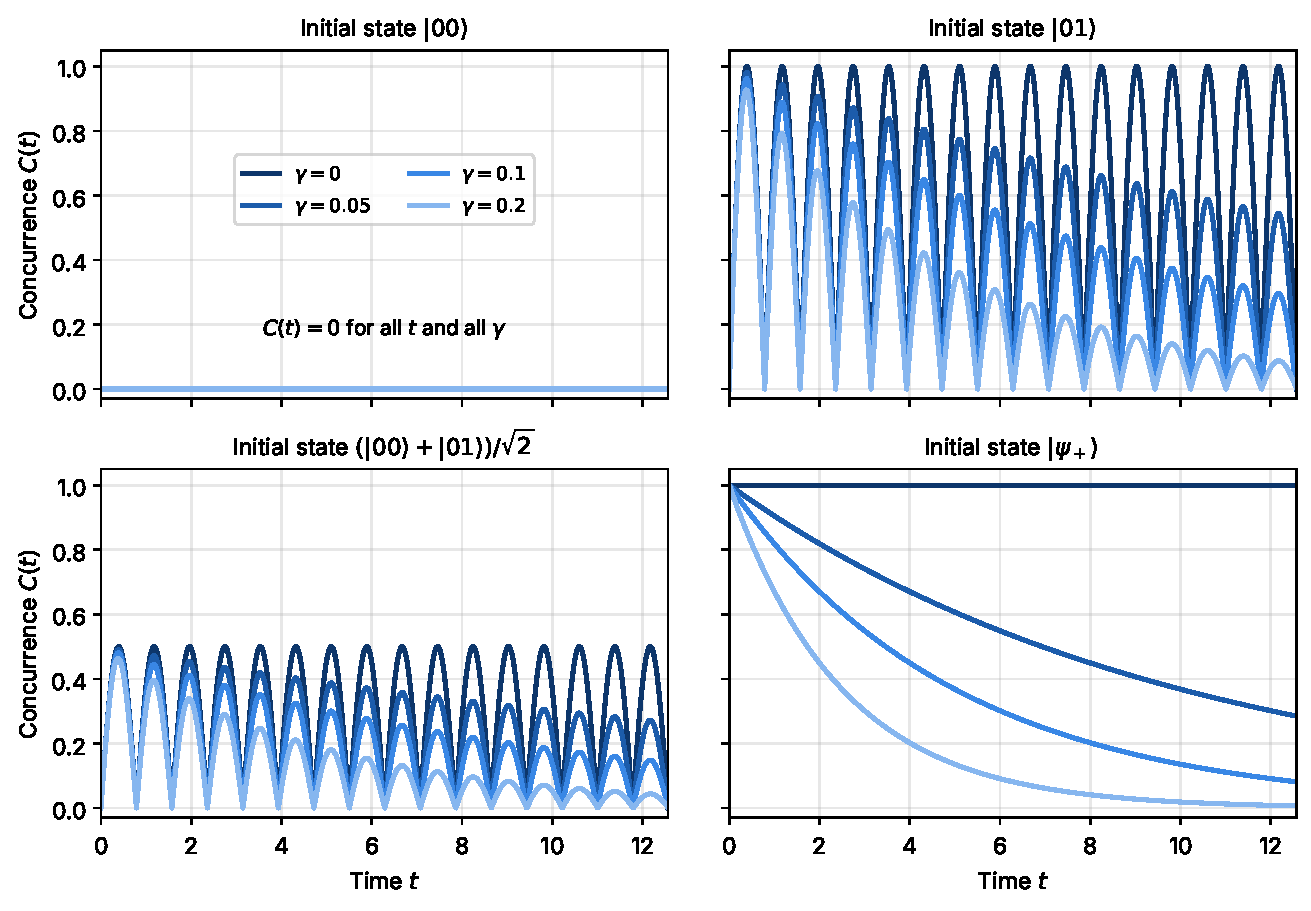
\includegraphics[width=0.85\textwidth]{nc_concurrence.pdf}
  \caption{Concurrence of the four initial states under local dephasing at $\lambda=0$, for $\gamma=0,\,0.05,\,0.1,\,0.2$ (dark to light).}
\end{figure}

No finite-time disentanglement (\emph{entanglement sudden death} \cite{YuEberly2004}) occurs for these states. The Bell state $\ket{\psi_+}$ loses its concurrence only asymptotically, as $e^{-2\gamma t}$. For $\ket{01}$ and $(\ket{00}+\ket{01})/\sqrt2$ the concurrence vanishes at the isolated nodes $\Omega t=k\pi$, as it already did without noise, and its envelope $e^{-\gamma t}$ decays smoothly.

\subsection{Quantum Fisher information under dephasing}
\figone{nc_state1_QFI.pdf}{Initial state $\ket{00}$: QFI for $V=S_x$ for several dephasing rates $\gamma$.}
\figone{nc_state2_QFI.pdf}{Initial state $\ket{01}$: QFI for $V=S_x$ for several dephasing rates $\gamma$.}
\figone{nc_state3_QFI.pdf}{Initial state $(\ket{00}+\ket{01})/\sqrt2$: QFI for $V=S_x$ for several dephasing rates $\gamma$.}
\figone{nc_state4_QFI.pdf}{Initial state $\ket{\psi_+}$: QFI for $V=S_x$ for several dephasing rates $\gamma$.}

\begin{table}[htbp]
  \centering
  \begin{tabular}{@{}lccccc@{}}
\toprule
Initial state & $\gamma=0$ & $\gamma=0.05$ & $\gamma=0.1$ & $\gamma=0.2$ & $\gamma=0.5$\\
\midrule
$\ket{00}$ & 8.00 & 6.88 & 5.97 & 4.62 & 2.47\\
$\ket{01}$ & 8.00 & 7.06 & 6.24 & 4.91 & 2.62\\
$(\ket{00}+\ket{01})/\sqrt2$ & 8.00 & 6.76 & 5.74 & 4.20 & 1.85\\
$\ket{\psi_+}$ & 16.00 & 13.65 & 11.61 & 8.46 & 3.72\\
\bottomrule
\end{tabular}

  \caption{Maximum over $t\in[0,4\pi]$ of the QFI, for $V=S_x$, $J=1$, $\Delta=0.5$.}
  \label{tab:nc-peak}
\end{table}

\subsubsection{Initial state $\ket{00}$}
Without noise $\FQ=8\sin^2(t/2)$ with peak value $8$ at $t=\pi$. Dephasing lowers the peak (Table~\ref{tab:nc-peak}) and moves it slightly to earlier times, from $t\simeq3.14$ at $\gamma=0$ to $t\simeq2.97$ at $\gamma=0.1$. At $\gamma=0.5$ the peak has dropped to $2.47$.

\subsubsection{Initial state $\ket{01}$}
At $\gamma=0$ the curve is identical to that of $\ket{00}$. With dephasing it is a few percent \emph{higher} than $\ket{00}$ (for instance $6.24$ against $5.97$ at $\gamma=0.1$), so among the two product states it is the more robust probe.

\subsubsection{Initial state $(\ket{00}+\ket{01})/\sqrt2$}
Its peak is $8$ at $\gamma=0$ but it is the most fragile of the product states, with $5.74$ at $\gamma=0.1$ and $1.85$ at $\gamma=0.5$. The coherence between the sectors $M=+1$ and $M=0$ is not protected against the $z$-dephasing.

\subsubsection{Initial state $\ket{\psi_+}$}
The QFI is $16\sin^2(t/2)$ at $\gamma=0$, with peak $16$. The peak decreases to $13.65$, $11.61$, $8.46$ and $3.72$ for $\gamma=0.05$, $0.1$, $0.2$ and $0.5$.

\subsubsection{Long-time behaviour}
For $t\gg1/\gamma$ the oscillations are damped and the QFI approaches a plateau that is the \emph{same} for $\ket{00}$, $\ket{01}$ and $\ket{\psi_+}$ (Table~\ref{tab:nc-plateau}). For $\Delta=0.5$ it is well described by
\begin{equation}
  \FQ(t\to\infty)=\frac{2}{\omega^2+\gamma^2}.
\end{equation}
We found this expression empirically and have not derived it. It agrees with the numerics to four digits for $\Delta=0,\,0.25,\,0.5,\,0.75$ and $\gamma=0.1,\,0.5$. The initial state is forgotten, so any advantage of the entangled state is a finite-time effect.

\begin{table}[htbp]
  \centering
  \begin{tabular}{@{}lccccc@{}}
\toprule
$\gamma$ & $\ket{00}$ & $\ket{01}$ & $(\ket{00}+\ket{01})/\sqrt2$ & $\ket{\psi_+}$ & $2/(\omega^2+\gamma^2)$\\
\midrule
0.05 & 1.995 & 1.995 & 1.660 & 1.995 & 1.995\\
0.1 & 1.980 & 1.980 & 1.640 & 1.980 & 1.980\\
0.2 & 1.923 & 1.923 & 1.566 & 1.923 & 1.923\\
0.5 & 1.600 & 1.600 & 1.173 & 1.600 & 1.600\\
\bottomrule
\end{tabular}

  \caption{QFI at $t=300$ ($\Delta=0.5$). The last column is the empirical expression $2/(\omega^2+\gamma^2)$.}
  \label{tab:nc-plateau}
\end{table}

\subsection{Cram\'er--Rao bound under dephasing}
With $N=1000$ repetitions, $\delta\lambda_{\min}(t)=1/\sqrt{N\FQ(t)}$ for the QFI of the previous subsection. The bound diverges at the nodes of $\FQ$, so the interrogation time must be chosen near a maximum.
\figpair{nc_state1_CRB.pdf}{nc_state2_CRB.pdf}{Cram\'er--Rao bound for the initial states $\ket{00}$ (left) and $\ket{01}$ (right).}
\figpair{nc_state3_CRB.pdf}{nc_state4_CRB.pdf}{Cram\'er--Rao bound for the initial states $(\ket{00}+\ket{01})/\sqrt2$ (left) and $\ket{\psi_+}$ (right).}
\begin{table}[htbp]
  \centering
  \begin{tabular}{@{}lccccc@{}}
\toprule
Initial state & $\gamma=0$ & $\gamma=0.05$ & $\gamma=0.1$ & $\gamma=0.2$ & $\gamma=0.5$\\
\midrule
$\ket{00}$ & 0.0112 & 0.0121 & 0.0129 & 0.0147 & 0.0201\\
$\ket{01}$ & 0.0112 & 0.0119 & 0.0127 & 0.0143 & 0.0196\\
$(\ket{00}+\ket{01})/\sqrt2$ & 0.0112 & 0.0122 & 0.0132 & 0.0154 & 0.0232\\
$\ket{\psi_+}$ & 0.0079 & 0.0086 & 0.0093 & 0.0109 & 0.0164\\
\bottomrule
\end{tabular}

  \caption{Best (smallest) value of $\delta\lambda_{\min}$ over $t\in[0,4\pi]$, for $N=1000$.}
\end{table}
Without noise the best values are $0.0112$ for $\ket{00}$ and $0.0079$ for $\ket{\psi_+}$, a gain of $\sqrt2$. At $\gamma=0.1$ they become $0.0129$ and $0.0093$, a gain of $1.39$. As before, the bound is attainable only with an optimal measurement, which we do not discuss here.

\subsection{Comparative discussion}
\begin{figure}[htbp]
  \centering
  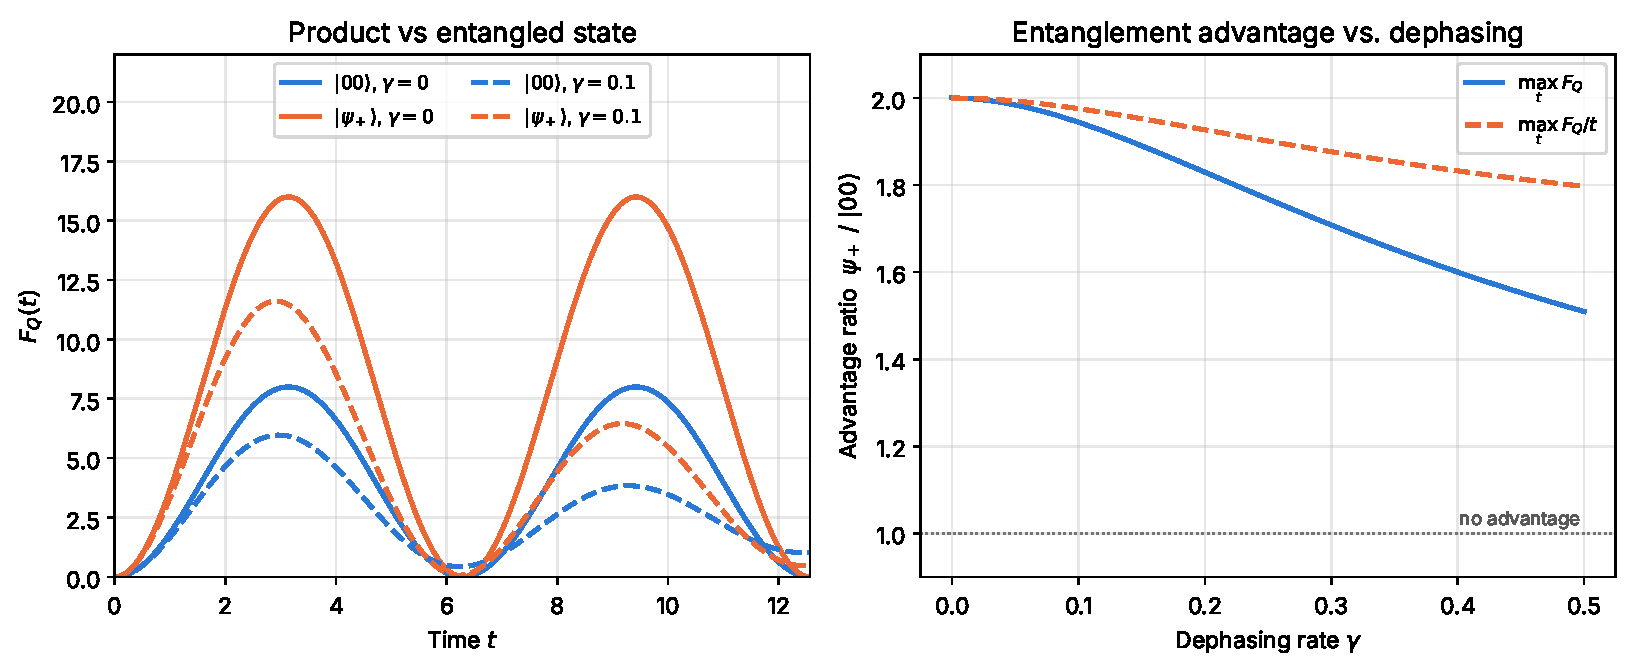
\includegraphics[width=\textwidth]{nc_comparison.pdf}
  \caption{Left: QFI of the product state $\ket{00}$ and of the Bell state $\ket{\psi_+}$ without noise (solid) and with dephasing $\gamma=0.1$ (dashed). Right: ratio between the best QFI of $\ket{\psi_+}$ and of $\ket{00}$ as a function of $\gamma$, for the maximum of $\FQ$ and for the maximum of $\FQ/t$.}
\end{figure}
\begin{table}[htbp]
  \centering
  \begin{tabular}{@{}lccc@{}}
\toprule
$\gamma$ & $\max_t F_Q$ ratio & $\max_t F_Q/t$ ratio & time fraction with $F_{\psi_+}>F_{00}$\\
\midrule
0 & 2.00 & 2.00 & 100\%\\
0.05 & 1.99 & 2.00 & 90\%\\
0.1 & 1.94 & 1.98 & 82\%\\
0.2 & 1.83 & 1.93 & 70\%\\
0.5 & 1.51 & 1.80 & 57\%\\
\bottomrule
\end{tabular}

  \caption{Entanglement advantage of $\ket{\psi_+}$ over $\ket{00}$. The last column is the fraction of $t\in(0,4\pi]$ at which $\FQ^{(\psi_+)}>\FQ^{(00)}$.}
  \label{tab:nc-adv}
\end{table}

The results can be summarised as follows.
\begin{enumerate}
  \item \textbf{Role of $\Delta$.} With a non-commuting generator the anisotropy enters the QFI through $\omega=2J(1-\Delta)$, unlike the commuting case of Sec.~\ref{sec:metrology}.
  \item \textbf{Noiseless advantage.} The Bell state gives exactly twice the QFI of the product states $\ket{00}$ and $\ket{01}$ at all times; in the isotropic limit this is the $N^2t^2$ against $Nt^2$ scaling for $N=2$.
  \item \textbf{The advantage survives dephasing at the best time, but shrinks.} The ratio of the maximal QFI decreases from $2.00$ to $1.94$, $1.83$ and $1.51$ for $\gamma=0.1$, $0.2$ and $0.5$. If the figure of merit is the information per unit time, $\max_t\FQ/t$, the advantage is more robust: $1.98$, $1.93$ and $1.80$.
  \item \textbf{No sudden death.} The concurrence of $\ket{\psi_+}$ decays as $e^{-2\gamma t}$ and does not vanish at any finite time.
  \item \textbf{Windows where the product state is better.} The product state $\ket{00}$ has a larger QFI than $\ket{\psi_+}$ during windows around the nodes of $\FQ$, where both are small; their total duration grows with $\gamma$ (the Bell state is ahead during $82\%$ of the interval at $\gamma=0.1$ and $57\%$ at $\gamma=0.5$). At the first maximum of the QFI the Bell state remains ahead for every $\gamma$ studied (Table~\ref{tab:nc-adv}).
  \item \textbf{Long times.} For $t\gg1/\gamma$ all initial states except $(\ket{00}+\ket{01})/\sqrt2$ reach the same plateau, and the advantage disappears.
\end{enumerate}
Hence, in this model, entanglement-enhanced sensitivity is \emph{degraded}, but not destroyed, by local dephasing, and the best strategy is to interrogate the system around the first maximum of $\FQ$, at a time of order $\pi/\omega$ or shorter, rather than at long times. This is qualitatively consistent with the known result that, under dephasing, the quantum advantage of entangled probes does not persist at long times and is limited to a constant factor \cite{Huelga1997,Escher2011,Demkowicz2012}. We stress that the present analysis is a two-qubit case study with pure initial states and one noise model; the ingredients are standard and the contribution is a fully checked, quantitative characterisation of these four states.

% ====================================================================
\section{Conclusion and Outlook}\label{sec:conclusion}
% ====================================================================

The two-qubit XXZ model is exactly solvable and its dynamics is organised by the conserved total $S_z$. Four initial states chosen to cover the sectors of the Hamiltonian give: no entanglement and no dynamics for $\ket{00}$; a full oscillation $C(t)=\lvert\sin4Jt\rvert$ for $\ket{01}$; a reduced oscillation $C(t)=\tfrac12\lvert\sin4Jt\rvert$ for $(\ket{00}+\ket{01})/\sqrt2$; and constant maximal entanglement for $\ket{\psi_+}$. The anisotropy $\Delta$ only appears as phases and does not alter $C$, $\mathcal N$ or the purities of these states. For the metrological problem, $[H,V]=0$ yields $\FQ=4t^2\Var(V)$, non-zero only for superpositions of different $S_z$ sectors.

With the non-commuting generator $V=S_x$, the QFI depends on $\Delta$ through $\omega=2J(1-\Delta)$: $\FQ=8\sin^2(\omega t/2)/\omega^2$ for $\ket{00}$ and $\ket{01}$, and exactly twice this for $\ket{\psi_+}$. Under local dephasing the concurrence decays without sudden death ($e^{-2\gamma t}$ for $\ket{\psi_+}$), the entanglement advantage of $\ket{\psi_+}$ decreases from a factor $2$ to $1.94$, $1.83$ and $1.51$ at the best time for $\gamma=0.1$, $0.2$, $0.5$, and for $t\gg1/\gamma$ the QFI of $\ket{00}$, $\ket{01}$ and $\ket{\psi_+}$ approaches the same plateau.

\paragraph{Limitations.} The initial states are pure, only one noise model (local pure dephasing in the $z$ basis) is considered, and the system has two qubits, so no scaling with the number of probes can be extracted. The long-time QFI plateau $2/(\omega^2+\gamma^2)$ is an empirical fit that has not been derived, and the Cram\'er--Rao bound is not shown to be attainable with a specific measurement.

\paragraph{Perspectives.} Natural extensions are: initial states with support on all sectors; other noise models (amplitude damping, depolarisation, correlated dephasing), for which sudden death may or may not occur; a derivation of the long-time plateau; the optimal measurement saturating the Cram\'er--Rao bound; larger chains ($N>2$ qubits) to test the scaling of the QFI; and thermal states of the XXZ model.

% ====================================================================
\appendix
\section{Hand calculations}
% ====================================================================
\subsection{Eigenvalues and eigenvectors of the XXZ Hamiltonian}

\paragraph{Step 1: block structure.}
In the basis $\{\ket{00},\ket{01},\ket{10},\ket{11}\}$ the Hamiltonian of Sec.~\ref{sec:dynamics} is
\begin{equation}
  H=J\begin{pmatrix}
  \Delta&0&0&0\\
  0&-\Delta&2&0\\
  0&2&-\Delta&0\\
  0&0&0&\Delta
  \end{pmatrix}.
\end{equation}
It is block diagonal: $\ket{00}$ and $\ket{11}$ are already eigenvectors with eigenvalue $J\Delta$, and the only block left to diagonalise is the $2\times2$ matrix acting on $\{\ket{01},\ket{10}\}$,
\begin{equation}
  H_0=J\begin{pmatrix}-\Delta&2\\2&-\Delta\end{pmatrix}.
\end{equation}

\paragraph{Step 2: characteristic equation.}
The eigenvalues $E$ are the roots of $\det(H_0-E\,I)=0$:
\begin{equation}
  \det\begin{pmatrix}-J\Delta-E&2J\\2J&-J\Delta-E\end{pmatrix}
  =(-J\Delta-E)^2-4J^2=0
  \quad\Longrightarrow\quad
  E_\pm=-J\Delta\pm2J .
\end{equation}

\paragraph{Step 3: eigenvectors.}
We solve the eigenvalue equation $H_0\begin{pmatrix}u\\v\end{pmatrix}=E\begin{pmatrix}u\\v\end{pmatrix}$. The first row reads $-J\Delta\,u+2J\,v=E\,u$ (the second row gives the same condition).
\begin{itemize}
  \item For $E_+=-J\Delta+2J$: $2Jv=2Ju$, hence $v=u$.
  \item For $E_-=-J\Delta-2J$: $2Jv=-2Ju$, hence $v=-u$.
\end{itemize}

\paragraph{Step 4: normalisation.}
Imposing $\lvert u\rvert^2+\lvert v\rvert^2=1$ gives $\lvert u\rvert=1/\sqrt2$ in both cases. Up to a global phase,
\begin{equation}
  \ket{\psi_\pm}=\frac{1}{\sqrt2}\bigl(\ket{01}\pm\ket{10}\bigr),\qquad H\ket{\psi_\pm}=(-J\Delta\pm2J)\ket{\psi_\pm}.
\end{equation}
Together with $\ket{00}$ and $\ket{11}$ this reproduces the spectrum of Table~1. The two eigenvectors are orthogonal, $\braket{\psi_+}{\psi_-}=\tfrac12(1-1)=0$, as required for a Hermitian matrix with distinct eigenvalues.

\subsection{Concurrence of a pure two-qubit state}

Let a general normalised pure state be
\begin{equation}
  \ket{\varphi}=c_{00}\ket{00}+c_{01}\ket{01}+c_{10}\ket{10}+c_{11}\ket{11},\qquad \sum_{ij}\lvert c_{ij}\rvert^2=1 .
\end{equation}

\paragraph{Separable states give $c_{00}c_{11}-c_{01}c_{10}=0$.}
A product state has the form
\begin{equation}
  \ket{\varphi}=(\alpha\ket{0}+\beta\ket{1})\otimes(\gamma\ket{0}+\epsilon\ket{1})
  =\alpha\gamma\ket{00}+\alpha\epsilon\ket{01}+\beta\gamma\ket{10}+\beta\epsilon\ket{11}.
\end{equation}
Comparing with the general expansion, $c_{00}=\alpha\gamma$, $c_{01}=\alpha\epsilon$, $c_{10}=\beta\gamma$ and $c_{11}=\beta\epsilon$, so
\begin{equation}
  c_{00}c_{11}-c_{01}c_{10}=\alpha\gamma\beta\epsilon-\alpha\epsilon\beta\gamma=0 .
\end{equation}
Conversely, if $c_{00}c_{11}=c_{01}c_{10}$, the coefficient matrix $\bigl(\begin{smallmatrix}c_{00}&c_{01}\\c_{10}&c_{11}\end{smallmatrix}\bigr)$ has zero determinant, hence rank one, its two rows are proportional and the state factorises. Therefore the quantity $\lvert c_{00}c_{11}-c_{01}c_{10}\rvert$ vanishes if and only if the state is separable, which motivates the definition
\begin{equation}
  C(\varphi)=2\,\lvert c_{00}c_{11}-c_{01}c_{10}\rvert .
\end{equation}

\paragraph{Why the factor $2$: the range is $[0,1]$.}
Using the triangle inequality and $2\lvert x\rvert\lvert y\rvert\le\lvert x\rvert^2+\lvert y\rvert^2$,
\begin{equation}
  \lvert c_{00}c_{11}-c_{01}c_{10}\rvert\le\lvert c_{00}\rvert\lvert c_{11}\rvert+\lvert c_{01}\rvert\lvert c_{10}\rvert
  \le\tfrac12\bigl(\lvert c_{00}\rvert^2+\lvert c_{11}\rvert^2\bigr)+\tfrac12\bigl(\lvert c_{01}\rvert^2+\lvert c_{10}\rvert^2\bigr)=\tfrac12 .
\end{equation}
So $\lvert c_{00}c_{11}-c_{01}c_{10}\rvert\in[0,\tfrac12]$, and the factor $2$ rescales the concurrence to $C\in[0,1]$. The maximum is reached by Bell states: for $\ket{\psi_+}$, $c_{01}=c_{10}=1/\sqrt2$ and $C=2\cdot\tfrac12=1$.

\paragraph{Consistency with Wootters' formula.}
For a pure state, $C=\lvert\langle\varphi\rvert\sigma_y\otimes\sigma_y\lvert\varphi^{*}\rangle\rvert$. Since $\sigma_y\otimes\sigma_y\ket{\varphi^{*}}=-c_{11}^{*}\ket{00}+c_{10}^{*}\ket{01}+c_{01}^{*}\ket{10}-c_{00}^{*}\ket{11}$, one finds $\langle\varphi\rvert\sigma_y\otimes\sigma_y\lvert\varphi^{*}\rangle=-2\bigl(c_{00}^{*}c_{11}^{*}-c_{01}^{*}c_{10}^{*}\bigr)$, whose modulus is $2\lvert c_{00}c_{11}-c_{01}c_{10}\rvert$, in agreement with the definition above.


\section{Numerical implementation}
% ====================================================================
All numerics use QuTiP \cite{QuTiP2012}; the code is organised as a small Python package (\texttt{xxz/}) with the scripts that regenerate every figure and table, and a validation script that runs all the checks below (see the repository \texttt{README}). Time evolution is done with \texttt{mesolve} (tolerances $10^{-13}$ and $10^{-11}$), with $J=1$, $\Delta=0.5$ and $N=1000$. Concurrence is computed with the Wootters formula and negativity from the eigenvalues of the partial transpose. The analytic $C(t)$, $\mathcal N(t)$ and purities of Sec.~\ref{sec:dynamics} agree with the numerical ones to $4\times10^{-8}$, and the analytic QFI of Eq.~\eqref{eq:FQ} agrees with a finite-difference derivative of the evolved state on a grid of times to $4\times10^{-6}$.

For Sec.~\ref{sec:noncomm}, the mixed-state QFI is computed from the eigendecomposition of $\rho$ with a central finite difference ($10^{-4}$) in $\lambda$. The following checks are run by \texttt{scripts/validate.py}: the QuTiP evolution agrees with an independent NumPy/SciPy implementation (exponentiation of the $16\times16$ Liouvillian) to $4\times10^{-10}$; at $\gamma=0$ the QFI agrees with the Duhamel formula~\eqref{eq:FQ-G} to $4\times10^{-6}$, and the Duhamel formula agrees with the closed forms~\eqref{eq:FQ-closed} to $10^{-14}$; for $\gamma>0$ the QFI agrees with a superoperator pseudo-inverse implementation to $10^{-15}$ and with a fidelity-based estimate to $2.4\times10^{-3}$; the closed-form concurrences agree with Wootters' formula to $7\times10^{-10}$; and the empirical plateau $2/(\omega^2+\gamma^2)$ holds to $10^{-5}$ for $\Delta=0,\,0.25,\,0.5,\,0.75$ and $\gamma=0.1,\,0.5$. The tables of Sec.~\ref{sec:noncomm} are generated by the same script that produces the figures.

% ====================================================================
\begin{thebibliography}{9}

\bibitem{Wootters1998} W.~K. Wootters, ``Entanglement of formation of an arbitrary state of two qubits,'' Phys.\ Rev.\ Lett.\ \textbf{80}, 2245 (1998).

\bibitem{VidalWerner2002} G.~Vidal and R.~F. Werner, ``Computable measure of entanglement,'' Phys.\ Rev.\ A \textbf{65}, 032314 (2002).

\bibitem{Horodecki2009} R.~Horodecki, P.~Horodecki, M.~Horodecki and K.~Horodecki, ``Quantum entanglement,'' Rev.\ Mod.\ Phys.\ \textbf{81}, 865 (2009).

\bibitem{BraunsteinCaves1994} S.~L. Braunstein and C.~M. Caves, ``Statistical distance and the geometry of quantum states,'' Phys.\ Rev.\ Lett.\ \textbf{72}, 3439 (1994).

\bibitem{Giovannetti2011} V.~Giovannetti, S.~Lloyd and L.~Maccone, ``Advances in quantum metrology,'' Nature Photon.\ \textbf{5}, 222 (2011).

\bibitem{Lindblad1976} G.~Lindblad, ``On the generators of quantum dynamical semigroups,'' Commun.\ Math.\ Phys.\ \textbf{48}, 119 (1976).

\bibitem{GKS1976} V.~Gorini, A.~Kossakowski and E.~C.~G. Sudarshan, ``Completely positive dynamical semigroups of $N$-level systems,'' J.\ Math.\ Phys.\ \textbf{17}, 821 (1976).

\bibitem{BreuerPetruccione2002} H.-P. Breuer and F.~Petruccione, \emph{The Theory of Open Quantum Systems} (Oxford University Press, 2002).

\bibitem{YuEberly2004} T.~Yu and J.~H. Eberly, ``Finite-time disentanglement via spontaneous emission,'' Phys.\ Rev.\ Lett.\ \textbf{93}, 140404 (2004).

\bibitem{Huelga1997} S.~F. Huelga, C.~Macchiavello, T.~Pellizzari, A.~K. Ekert, M.~B. Plenio and J.~I. Cirac, ``Improvement of frequency standards with quantum entanglement,'' Phys.\ Rev.\ Lett.\ \textbf{79}, 3865 (1997).

\bibitem{Escher2011} B.~M. Escher, R.~L. de~Matos~Filho and L.~Davidovich, ``General framework for estimating the ultimate precision limit in noisy quantum-enhanced metrology,'' Nature Phys.\ \textbf{7}, 406 (2011).

\bibitem{Demkowicz2012} R.~Demkowicz-Dobrza\'nski, J.~Ko\l ody\'nski and M.~Gu\c{t}\u{a}, ``The elusive Heisenberg limit in quantum-enhanced metrology,'' Nat.\ Commun.\ \textbf{3}, 1063 (2012).

\bibitem{QuTiP2012} J.~R. Johansson, P.~D. Nation and F.~Nori, ``QuTiP: An open-source Python framework for the dynamics of open quantum systems,'' Comput.\ Phys.\ Commun.\ \textbf{183}, 1760 (2012).

\end{thebibliography}

\end{document}
